\documentclass[12pt]{report}

\usepackage[english]{babel}
\usepackage[utf8x]{inputenc}
\usepackage{amsmath}
\usepackage{graphicx}
\usepackage{multirow}
\usepackage[hypcap]{caption}
\usepackage{setspace} 
\usepackage{float}

\title{Lab 9: Composite Materials}
\author{Zachary Tschirhart \\
	\small \\
        \small EID: zst75 \\
	\small Department of Aerospace Engineering and Engineering Mechanics \\
	\small \textbf{ASE 324L (Mon 2:00-5:00)} \\
	\small Unique: 13740}

\date{April 5, 2014}


\begin{document}
\maketitle

\begin{abstract}
Carbon fiber epoxy matrix material was tested in order to determine a generalized matrix. This resulting matrix could then be used to describe the composite's strength with several different orientations of the fibers and volumes of matrix. The loads were tensile and applied at a steady rate of strain for the three specimen of different fiber orientations. The fiber orientations were at zero, forty-five, and ninety degrees with respect to the applied stress. The dimensions of each specimen were known as well as the stress, axial strain, and transverse strain, which were found through the testing apparatus. This allowed for the calculation of Young's modulus and Poisson's ratio. Each of these calculated values were used to build the generalized compliance matrix that could then be used to estimate responses for a similar composite material with fibers laid in different orientations. Results were consistent with predictions as the zero degree fiber orientation provided the highest strength properties relative to the other two orientations tested.
\end{abstract}


\tableofcontents
\pagebreak

\setcounter{secnumdepth}{0}

\section{Introduction}
\doublespacing
Composite materials have unique properties, one of which includes a high strength to weight ratio. The specific composite material that has this property is the carbon fiber epoxy matrix material that was tested in this lab. Composite materials can reduce the weight required to create a stable structure if used properly; specifically, in the case of carbon fiber, the fibers must be oriented correctly and the structure analyzed to know the behaviors of the stresses being applied. This experiment tested three different orientations of carbon fiber material, which allowed for a general understanding of the orthotropic response to stresses. 

\section{Experimental and Data Reduction Procedures}
\subsection{Apparatus}
The apparatus used to provide a tensile stress to each specimen was a testing machine which provided a constant rate of strain change in the axial direction. In order to measure the strain in both the axial and transverse directions, extensometers were attached to each specimen and measured using a Wheatstone bridge. The voltages recorded by the Wheatstone bridge were then converted to strain by a calibration value.


\subsection{Procedure}
A total of six specimen were tested, of which only three unique configurations existed. The three unique configurations differed in the orientation of the fibers with respect to the stress being applied. The first specimen had the fibers parallel to the stress being applied, which can be referred to as the zero degree orientation. The second specimen had the fibers at plus and minus forty-five degrees from the applied stress, which can be referred to as the forty-five degree orientation. Lastly, a specimen with the fibers oriented perpendicular to the applied stress, referred to as the ninety degree orientation. Two series of tests were performed, of which all three orientations were tested.
Firstly, a tension test was performed on all three carbon fiber specimen with fibers oriented in the zero, forty-five, and ninety degree angles. This test allowed the three specimen to be loaded until failure occurred. These specimen had no sensors to measure the strain on the specimen. 
Secondly, the three specimen were loaded for a short time to gather the stress and strains in a small region without failure. These specimen had the sensors to measure stain both in the axial and transverse orientations. 

\subsection{Data Reduction}
The data collected from the testing apparatus was the load applied and cross-head displacement. Using the measured cross-sectional area of each specimen and the measured load, a stress could be calculated by the equation:

\begin{equation}
\begin{split}
  \sigma = \frac{P}{A}
  \label{equation:equation1}
\end{split}
\end{equation}

Where P is the applied load and A is the cross-sectional area. In order to convert the voltages into strain, the equation below was used:

\begin{equation}
\begin{split}
  \varepsilon = C*V
  \label{equation:equation2}
\end{split}
\end{equation}

Where C is the calibration factor and V is the voltage measured across the resistor. Now using the converted data, the Young's modulus could be found by calculating the slope of a stress-strain diagram, which is described by Hook's Law:

\begin{equation}
\begin{split}
  \sigma = E*\varepsilon
  \label{equation:equation3}
\end{split}
\end{equation}
\\

Where E is the Young's modulus. In order to get Poisson's ratio, the slope of the transverse versus axial strain was measured, which is describe by this equation:


\begin{equation}
\begin{split}
  \nu = -\frac{\varepsilon_t}{\varepsilon_a}
  \label{equation:equation4}
\end{split}
\end{equation}

Where \(\varepsilon_t\) is the strain in the transverse direction and \(\varepsilon_a\) is the strain the axial direction. In order to complete the compliance matrix, the shear modulus needed to be calculated for the forty-five degree fiber orientation. This can be calculated using the following:

\begin{equation}
\begin{split}
  G = \frac{E}{2(1-\nu)}
  \label{equation:equation5}
\end{split}
\end{equation}

Where the variables in the equation were all defined above. 

\section{Results and Discussion}
\doublespacing

Figures one through three display the measured stress versus strain plots used to calculate the Young's moduli for each specimen. Figures four though six display the transverse versus axial strain for each specimen, which is used to calculate the Poisson's ratio. The calculated values that are needed to find the compliance matrix are listed in the figure seven. Lastly, the calculated compliance matrix is displayed as equation 6.

\begin{figure}[H]
	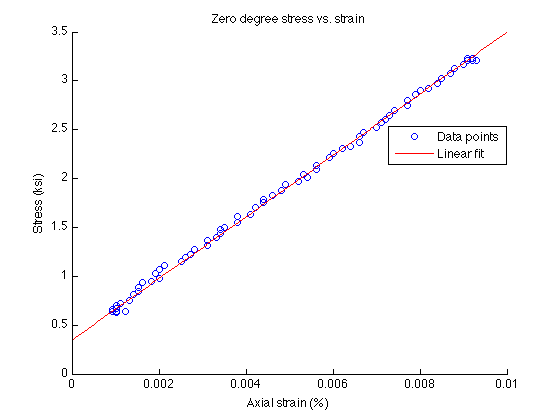
\includegraphics[width=1\textwidth]{0-stressvsstrain.png}
	\caption{Zero degree stress versus strain diagram}
	\label{fig:Figure1}
\end{figure}

\begin{figure}[H]
	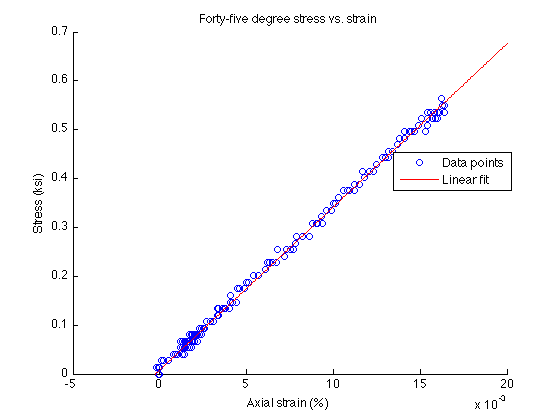
\includegraphics[width=1\textwidth]{45-stressvsstrain.png}
	\caption{Forty-five degree stress versus strain diagram}
	\label{fig:Figure2}
\end{figure}

\begin{figure}[H]
	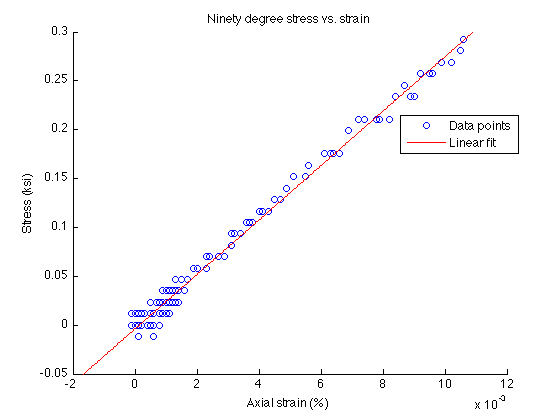
\includegraphics[width=1\textwidth]{90-stressvsstrain.png}
	\caption{Ninety degree stress versus strain diagram}
	\label{fig:Figure3}
\end{figure}


\begin{figure}[H]
	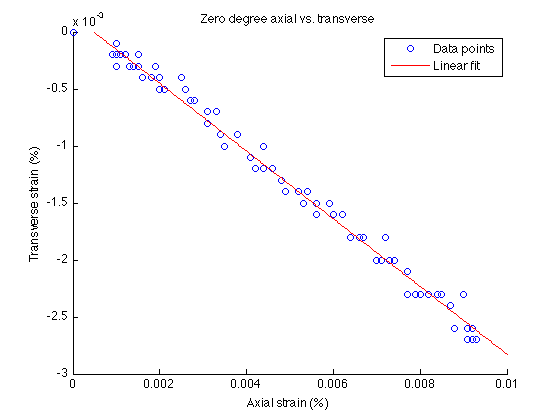
\includegraphics[width=1\textwidth]{0-poisson.png}
	\caption{Zero degree transverse versus axial strain diagram}
	\label{fig:Figure4}
\end{figure}

\begin{figure}[H]
	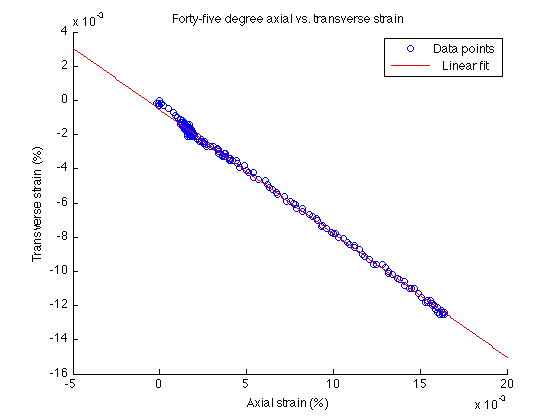
\includegraphics[width=1\textwidth]{45-poisson.png}
	\caption{Forty-five degree transverse versus axial strain diagram}
	\label{fig:Figure5}
\end{figure}

\begin{figure}[H]
	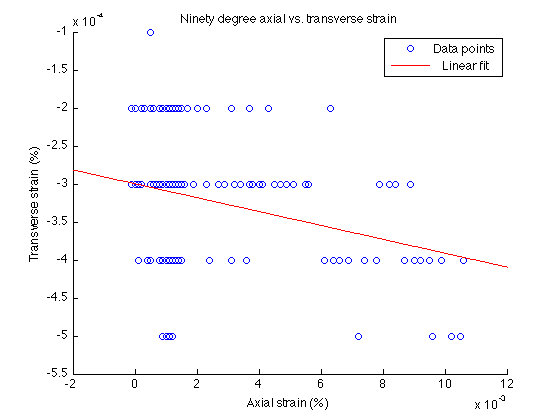
\includegraphics[width=1\textwidth]{90-poisson.png}
	\caption{Ninety degree transverse versus axial strain diagram}
	\label{fig:Figure6}
\end{figure}

\\
\\
\begin{figure}[H]
    \singlespacing
    \begin{tabular}{| p{3.2cm} | p{4cm}| p{3cm} | }
    \hline
    Fiber orientation (deg) & Young's modulus (ksi) & Poisson's ratio \\ \hline
    Zero       & 314.094 & 0.297 \\ \hline
    Forty-five &  33.387 & 0.724 \\ \hline
    Ninety     &  27.854 & 0.009 \\ \hline
    \end{tabular}
    \caption{Young's modulus and Poisson's ratio for the different fiber orientations}
\end{figure}\\
\doublespacing

\begin{equation}
\left[ 
  \begin{array}{c} 
    \varepsilon_1 \\ 
    \varepsilon_2 \\
    \gamma
  \end{array} 
\right] = 
\begin{bmatrix} 
  0.00318  & -0.00033 & 0 \\ 
  -0.00095 & 0.03590  & 0 \\
  0        & 0        & 0.10325
\end{bmatrix} \times 
\left[ 
  \begin{array}{c} 
    \sigma_1 \\ 
    \sigma_2 \\
    \sigma_{12} 
  \end{array} 
\right]
\caption{Compliance matrix}
\end{equation}
\\

\section{Micromechanics Analysis}
According to the laboratory manual, micromechanics is he study of composite material behavior wherein the interaction of the constituent materials is examined on a microscopic scale. Micromechanics is used as a volumetric analysis based on the volume of fibers and matrix material to determine theoretical values for the compliance matrix. As demonstrated below, expressions for \(E_1\), \(E_2\), \(\nu_{12}\), and \(G_{12}\) can be manipulated to estimate the volume of fibers based on the volume fraction of fibers versus matrix material.

Manipulating the rules of mixture equations in the lab manual, the following is found:
\begin{equation}
\begin{split}
  V_f = \frac{E_1 - E_m}{E_f - E_m}
  \label{equation:equation6}
\end{split}
\end{equation}

\begin{equation}
\begin{split}
  V_f = \frac{\frac{1}{E_2} - \frac{1}{E_m}}{\frac{1}{E_f} - \frac{1}{E_m}}
  \label{equation:equation7}
\end{split}
\end{equation}

\begin{equation}
\begin{split}
  V_f = \frac{\nu_1 - \nu_m}{\nu_f - \nu_m}
  \label{equation:equation8}
\end{split}
\end{equation}

\begin{equation}
\begin{split}
  V_f = \frac{\frac{1}{G_{12}} - \frac{1}{G_m}}{\frac{1}{G_f} - \frac{1}{G_m}}
  \label{equation:equation9}
\end{split}
\end{equation}

Then using the equations to relate Young's modulus and Poisson's ratio to Shear modulus,

\begin{equation}
\begin{split}
  G_m = \frac{E_m}{2(1+\nu_m)}
  \label{equation:equation10}
\end{split}
\end{equation}

\begin{equation}
\begin{split}
  G_f = \frac{E_f}{2(1+\nu_f)}
  \label{equation:equation11}
\end{split}
\end{equation}

Finally using the following equation, there are 7 equations for 7 unknowns,

\begin{equation}
\begin{split}
  \nu_{21} = V_f^3(\nu_f - \nu_m)(E_f - E_m)(\frac{1}{E_f} - \frac{1}{E_m}) + \\
             V_f^2(\nu_f - \nu_m)(E_f - E_m)(\frac{1}{E_m}) + \\
             V_f^2E_m(\nu_f - \nu_m)(\frac{1}{E_f} - \frac{1}{E_m}) + \\
             V_f^2\nu_m(E_f - E_m)(\frac{1}{E_f} - \frac{1}{E_m}) + \\
             V_f(\nu_f - \nu_m) + V_f\nu_m(E_f - E_m)(\frac{1}{E_m}) + \\
             V_f\nu_mE_m(\frac{1}{E_f} - \frac{1}{E_m}) + \nu_m
  \label{equation:equation12}
\end{split}
\end{equation}

Now solving the equations for the volume ratio of fibers, a value of 0.27456 is found, while 0.72544 is found for the volume ratio of the matrix material. 

\section{Conclusion}
\doublespacing
In conclusion, it was found that the carbon fiber material is strongest when the fibers are oriented parallel to the load being applied. Although the other orientations do not provide the highest tensile strength, they may be used for other applications and finding the compliance matrix will help determine the optimal fiber orientation without the need to experiment with every permutation. Moreover, a stress analysis of the applied usage is needed before using a material as complex as carbon fiber, as to not have an unexpected failure.


\begin{thebibliography}{0}
\bibitem{notes} {\em ASE 324L Lab manual : The University of Texas at Austin Department of Aerospace Engineering}  2014.
\bibitem{notes} {\em ASE 324L Lecture 17 : The University of Texas at Austin Department of Aerospace Engineering}  2014.
\bibitem{notes} {\em ASE 324L Lecture 18 : The University of Texas at Austin Department of Aerospace Engineering}  2014.
\end{thebibliography}
\addcontentsline{toc}{section}{Bibliography}


\end{document}
